% Page Setup -----------------------------------------------------
\documentclass[11pt, a4paper, fleqn, oneside]{article}
\usepackage[a4paper]{geometry}
\geometry{verbose,tmargin=1in,bmargin=1in,lmargin=.6in,rmargin=.6in}
% Packages ------------------------------------------------------
\usepackage{amsmath}
\usepackage{amsfonts}
\usepackage{hyperref}
\usepackage{lastpage}
\usepackage{setspace}
\usepackage{graphicx}
\usepackage{enumitem}
\setlist[description]{leftmargin=\parindent,labelindent=\parindent}
\usepackage{multicol}
\raggedcolumns
\usepackage{listings} 
\lstset{showstringspaces=false, frame=single, basicstyle=\footnotesize}
% Head / Foot ----------------------------------------------------
\usepackage{fancyhdr}
\setlength{\headheight}{15.2pt}
\pagestyle{fancy}
\lhead{}
\chead{CSCI3180 Principles of Programming Languages, Spring 2015-2016\\}
\rhead{Assignment 2 Report}
\rfoot{\today}
\cfoot{ }
\lfoot{Page \thepage\ of \pageref{LastPage}}

\begin{document}
\section{Polymorphism}
In traditional OOP, polymorphism relies on the inheritance tree to guarantee
certain functionality for a given object. Consider the following example, 
on the left we have inheritance-based polymorphism and on the right we have
duck-typing.\\
\begin{center}
    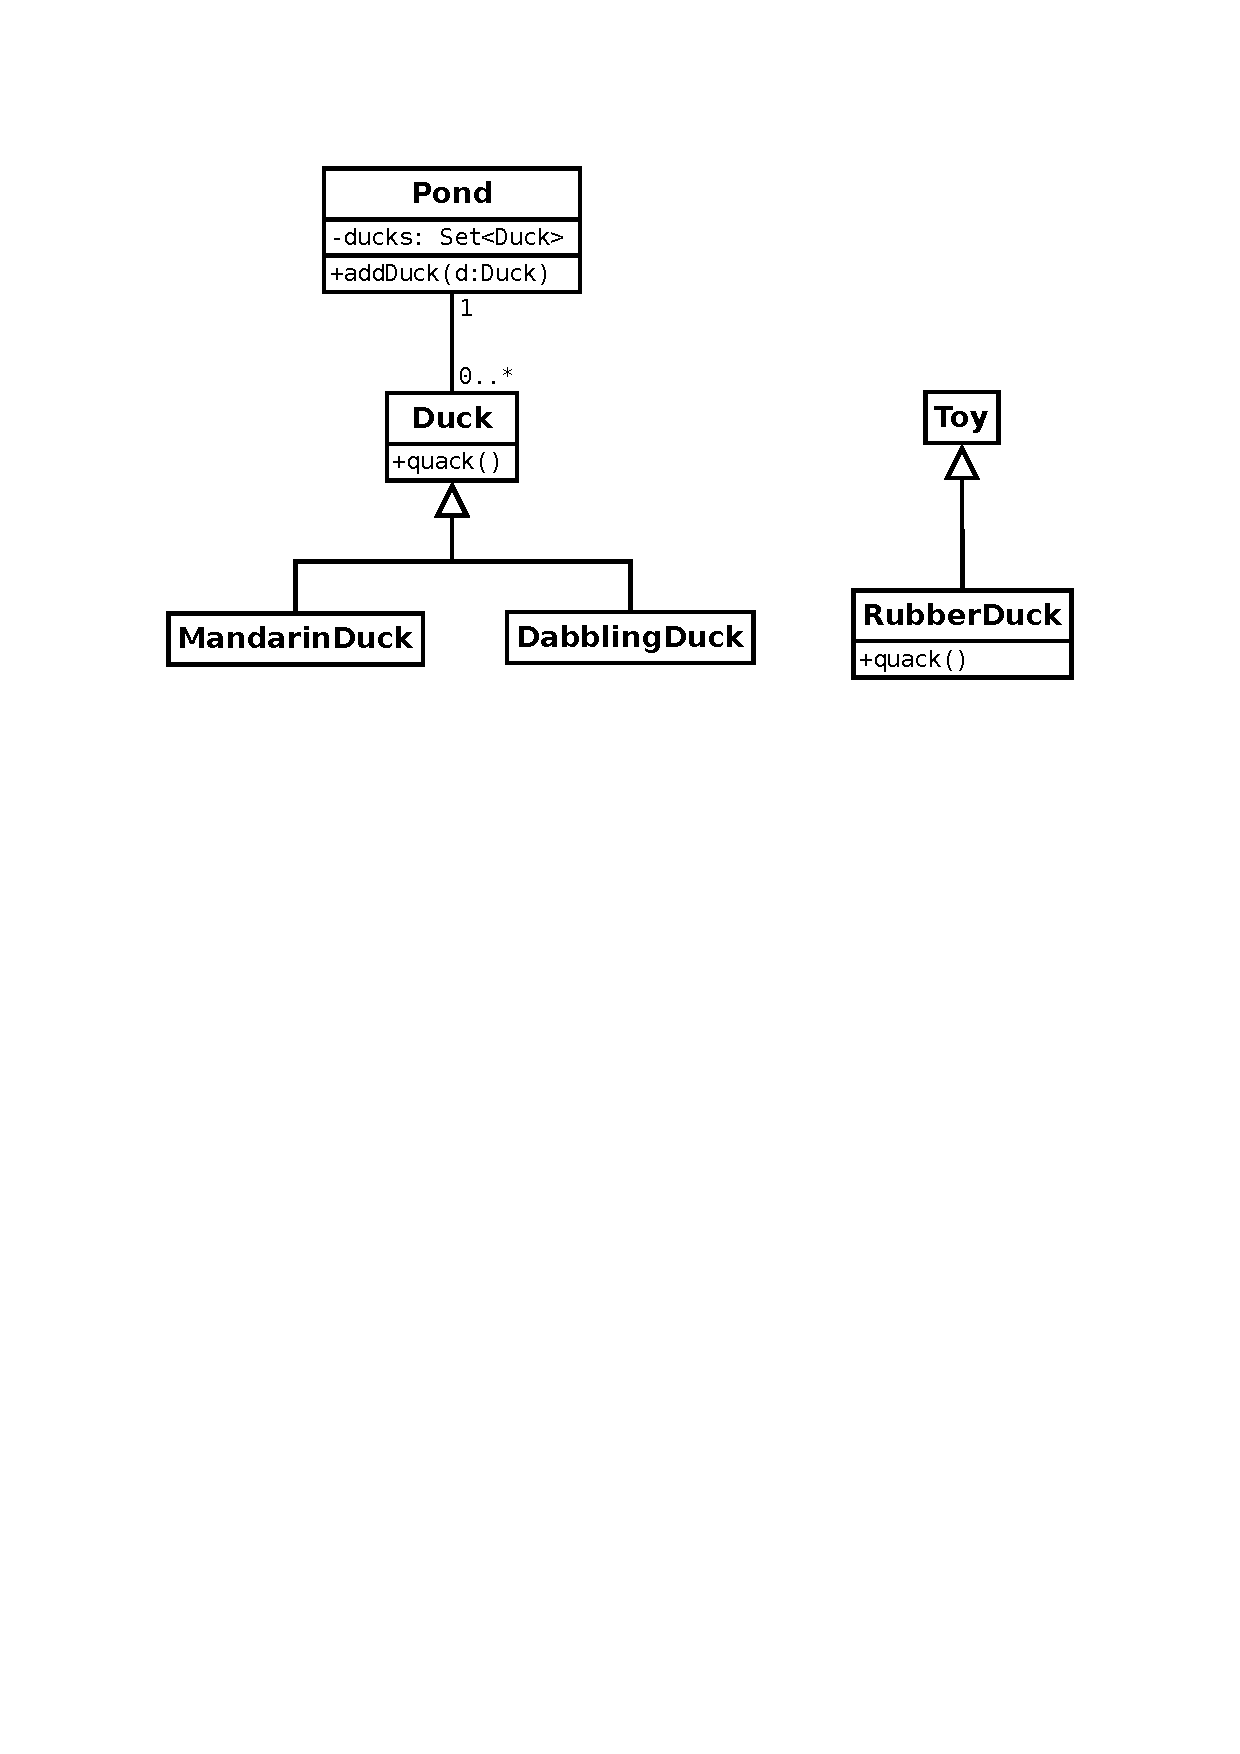
\includegraphics[trim=25mm 170mm 25mm 25mm, clip, width=0.48\textwidth]{duck1}
    \rule{.1pt}{60mm}
    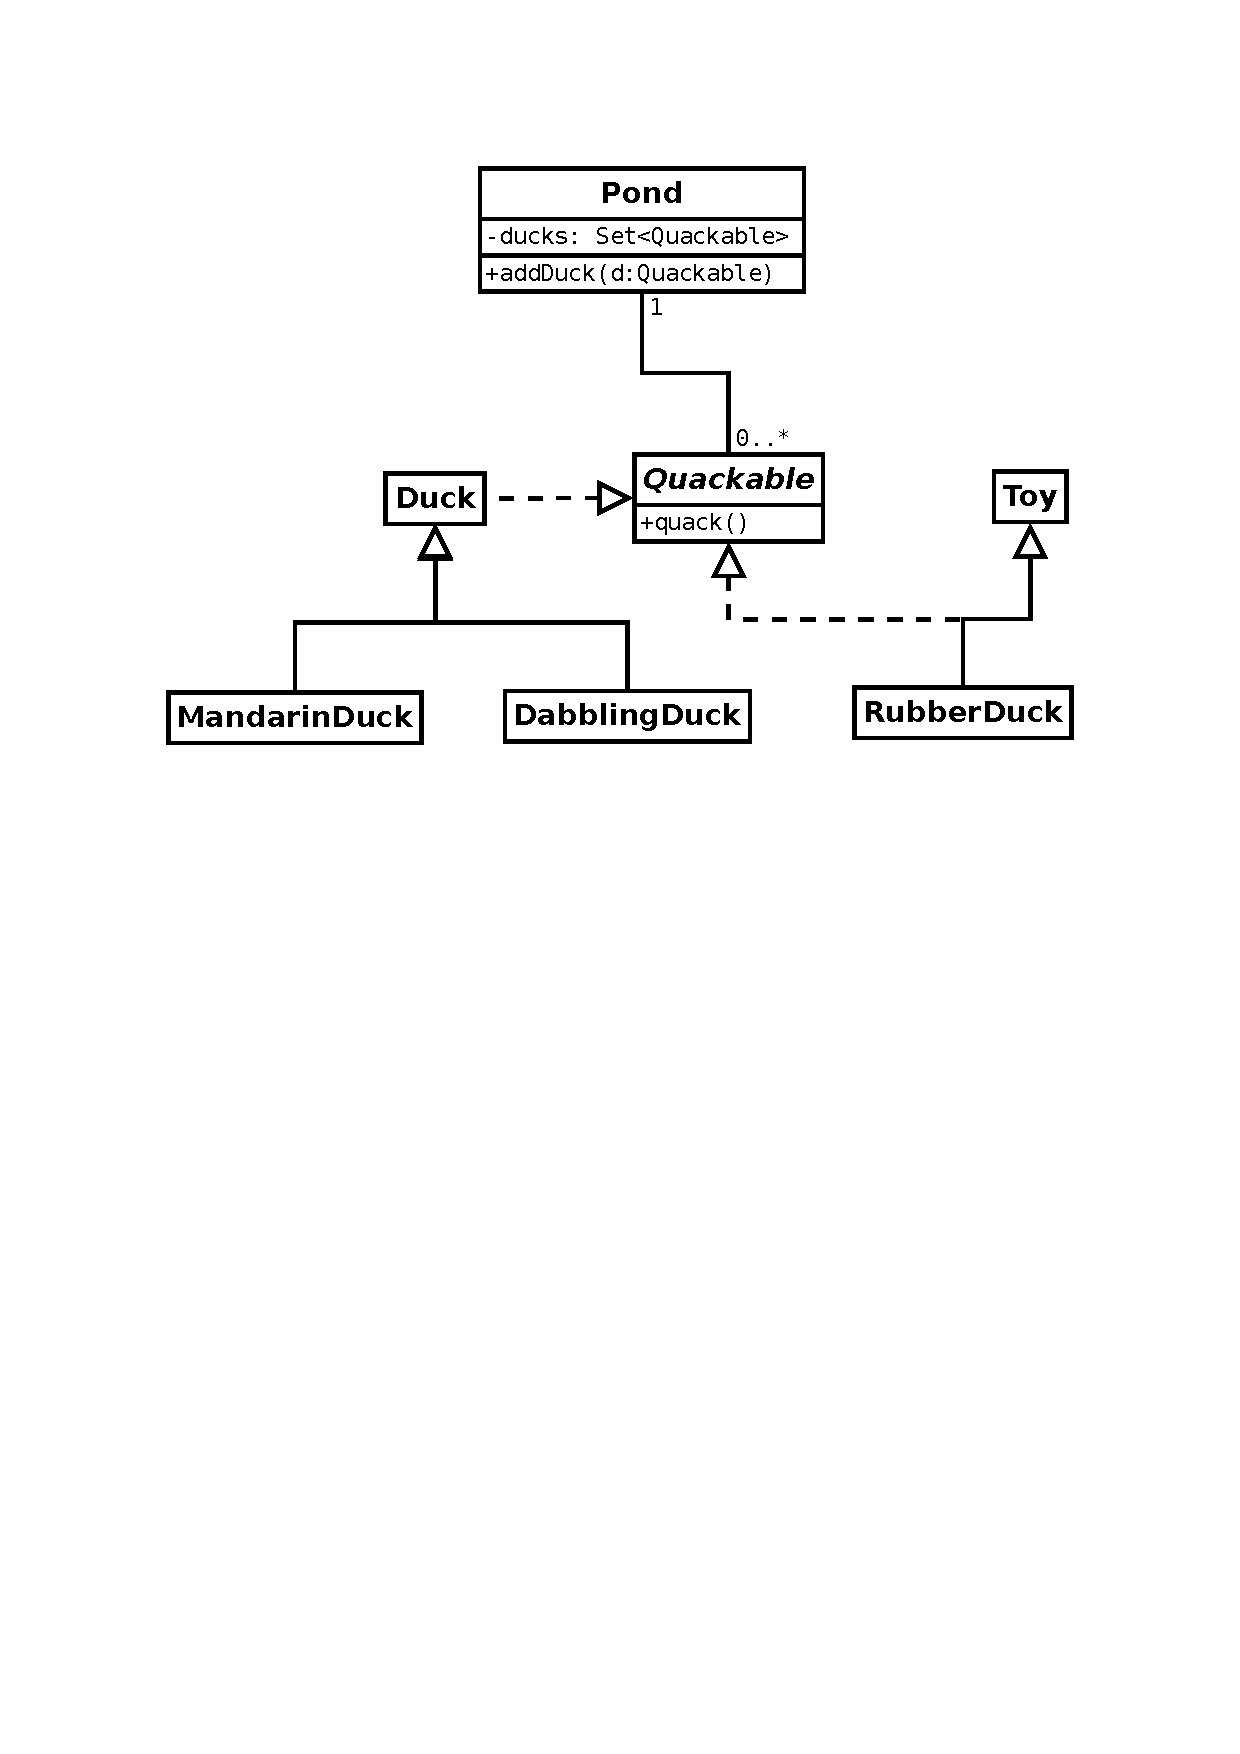
\includegraphics[trim=25mm 160mm 25mm 25mm, clip, width=0.48\textwidth]{duck2}
\end{center}
With inheritance, a RubberDuck cannot be added to the Pond even though it could quack like a Duck
because it doesn't inherit from the Duck class. However, with duck-typing, such
functionality guarantees can be delegated to mixins (AKA: interfaces, traits).
Now anything that behaves like a duck can be added to the Pond (i.e. can quack).
In Ruby and other languages with reflection, you can go one step further by
checking for a given functionality at runtime.

\section{Ruby vs Java}
Duck-typing support in Java is weaker than Ruby because mixins (interface with default methods)
does not have access to fields and methods in the implementing class. Compare the FoodBuyer
mixin in Ruby and Java below:
\begin{lstlisting}[language=Ruby]
module FoodBuyer
    def buyFood(foodName, cost)
        puts "Buy #{foodName} and pay $#{cost}."
        pay(cost)
    end
end
\end{lstlisting}
\begin{lstlisting}[language=Java]
interface FoodBuyer {
    public Consumer<Integer> pay();
    default public void buyFood(String foodName, int cost, Consumer<Integer> pay) {
        out.printf("Buy %s and pay $%d.\n", foodName, cost);
        pay.accept(cost);
    }
}
\end{lstlisting}\\
In the Java mixin, the buyFood method needs an extra `pay' closure to deligate
the pay operation to the implementing class because it does not have direct access unlike Ruby.

\end{document}
